\documentclass[a4paper,norsk]{article}
\usepackage[utf8]{inputenc}
\usepackage[T1]{fontenc,url}
\usepackage{babel,textcomp}
\usepackage{graphicx}
\usepackage{amsmath}
\usepackage{cleveref}
\usepackage[cmyk]{xcolor}
\usepackage{listings}
\graphicspath{ {./images/} }
\lstset {language=C++,    
backgroundcolor=\color{yellow!20},    
commentstyle=\color{green},    
%keywordstyle=\color{blue},    
basicstyle=\footnotesize}
\urlstyle{sf}
\title{Matte 3 Oblig 2}
\date{\today}
\author{Sivert Kindberg}
\newpage
\begin{document}
\maketitle
\tableofcontents
\newpage
 \section{Github}


\section{Oppgave 3.4.6}
Oppgave 3.4.6
utregningene er gjort i Excel \newline
Valgte punkter: (3, 10), ( 1, 6.5), (-5.9, 7.6), (-3, 5), (-2, 1.7), (-7, 4.3), (6.9, 4.2), (3.8, 5.2)\newline
\newline
y = Ax + e 
\newline
\begin{equation*} 
\begin{bmatrix}10 \\ 6.5\\7.6\\5\\1.7\\4.3\\4.2\\5.2\end{bmatrix}
=\begin{bmatrix}9 & 3 & 1 \\ 1 & 1 & 1 \\34.81 & -5.9 & 1 \\ 9 & -3 & 1 \\4 & -2 & 1 \\49& 7 & 1 \\47.61 & 6.9 & 1 \\ 14.9 & 3.8 & 1\end{bmatrix}\begin{bmatrix}a\\b\end{bmatrix}
+ \begin{bmatrix} e_1 \\ e_2 \\ e_3 \\ e_4 \\ e_5 \\ e_6 \\ e_7\end{bmatrix}
\end{equation*}


\begin{equation*}
B = A^{T} * A = \begin{bmatrix} 9 & 1 & 34.81 & 9 & 4 & 49 & 47.61 & 14.9 \\  3 & 1 & -5.9 & -3 & -2 & 7 & 6.9 & 3.8 \\1 & 1 & 1 & 1& 1 & 1 & 1 & 1\end{bmatrix}
\begin{bmatrix}  9 & 3 & 1 \\ 1 & 1 & 1 \\ 34.81 & -5.9 & 1 \\  9 & -3 & 1 \\4 & -2 & 1  \\49 & 7 & 1 \\47.61 & 6.9 & 1 \\ 14.9 & 3.8 & 1\end{bmatrix}
=\begin{bmatrix} 6280.4582 & 515.75 & 169.32 \\ 515.75 & 168.86 & 10.8 \\ 169.32 & 10.8 & 8\end{bmatrix}
\end{equation*} 


\begin{equation*}
C = A^{T} * y = \begin{bmatrix} 9 & 1 & 34.81 & 9 & 4 & 49 & 47.61 & 14.9 \\  3 & 1 & -5.9 & -3 & -2 & 7 & 6.9 & 3.8 \\1 & 1 & 1 & 1& 1 & 1 & 1 & 1 \end{bmatrix}
\begin{bmatrix}10 \\ 6.5\\7.6\\5\\1.7\\4.3\\4.2\\5.2\end{bmatrix}
=\begin{bmatrix}900.998 \\52.1 \\44.5 \end{bmatrix}
\end{equation*}

\begin{equation*}
B^{-1} = \begin{bmatrix} 0.000462474 & -0.000860823 & -0.008626157\\ -0.000860823 & 0.008084009 & 0.007305914 \\-0.008626157 & 0.007305914 & 0.297709637  \end{bmatrix}
\end{equation*}


\begin{equation*}
x = B^{-1} * c = \begin{bmatrix}  6280.4582 & 515.75 & 169.32 \\ 515.75 & 168.86 & 10.8 \\ 169.32 & 10.8 & 8  \end{bmatrix}\begin{bmatrix} 900.998 \\52.1 \\44.5 \end{bmatrix}
= \begin{bmatrix}-0.012024466 \\ -0.029310073 & 5.856566423 \end{bmatrix}
\end{equation*}

$y =-0.012024466x^{2}-0.029310073x+5.856566423$
\section{Beregne punkter og lagre i array}
Funksjonen tar inn x som verdi og bruker funksjonen fra utergningen og returnerer y verdien punktet skal ha.
\begin{lstlisting}[language=C++, caption={trianglesurface.h}]
static float func2(float x) {
       return 0.174 * x + 1, 743;
   }
\end{lstlisting}
\section{3.4.6 Visualisering}
VisualPoint klassen tar inn en vector av Vertexer, vertexene blir vist som hvite kvadrater.. MMap får en QuadraticPolynomial som tegner den grønne kurven.
\begin{lstlisting}[language=C++, caption={renderwindow.cpp}]
    mMap.insert(std::pair<std::string, VisualObject*>{"QuadtraticPolynomial", new QuadtraticPolynomial(-0.012024466, -0.029310073f, 5.856566423f, 0.1f)});
    std::vector<Vertex> points;
    points.push_back(Vertex{ 3, 10, 0 });
    points.push_back(Vertex{ 1, 6.5, 0 });
    points.push_back(Vertex{ -5.9, 7.6, 0 });
    points.push_back(Vertex{ -3, 5, 0 });
    points.push_back(Vertex{ -2, 1.7, 0 });
    points.push_back(Vertex{ -7, 4.3, 0 });
    points.push_back(Vertex{ 6.9, 4.2, 0 });
    points.push_back(Vertex{ 3.8, 5.2, 0 });

    for (auto i = 0; i < points.size(); i++) 
    {
        mMap.insert(std::pair<std::string, VisualObject*>{ std::to_string(i), new VisualPoint(points)});
    }
    }

\centering
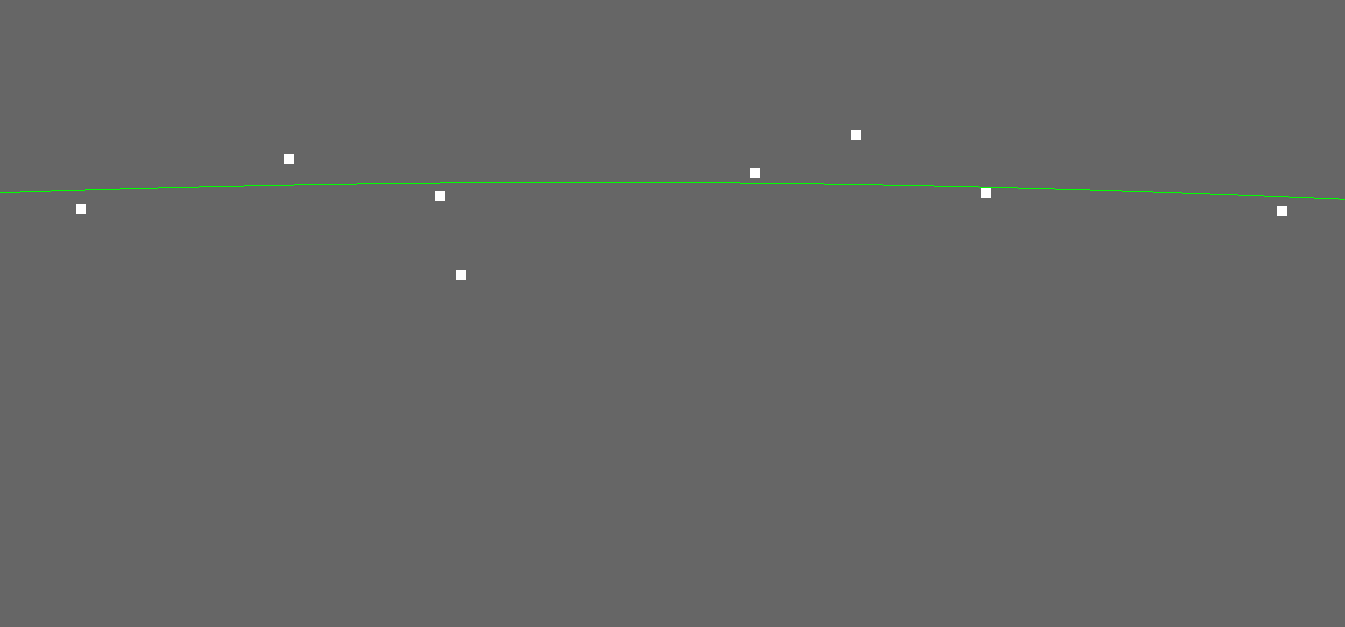
\includegraphics[width=\textwidth]{kurve1}
\end{lstlisting}
\end{document}